\documentclass[letterpaper]{amsart}
\usepackage{amsmath, amsthm, amsfonts, amsbsy, thmtools, amssymb,bm,xfrac,stmaryrd,mathrsfs,bbm}
\usepackage{tikz}
\usetikzlibrary{arrows}

\begin{document}

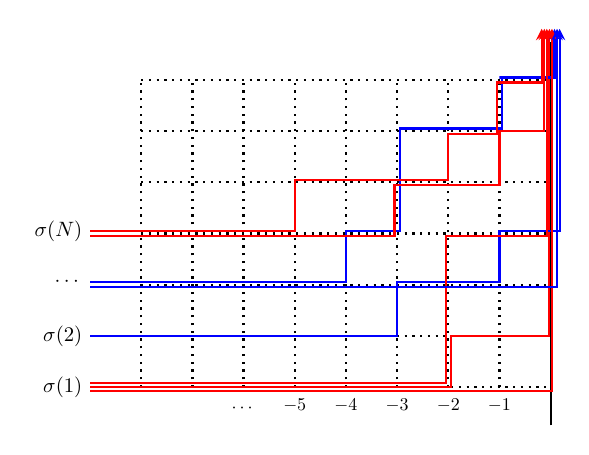
\begin{tikzpicture}[
	>=stealth, 
	scale = .65]{


		\draw[thick] (23, -.25) -- (23, 7.25);

		\draw[black, thick, dotted] (15, .5) -- (15, 6.5);
		\draw[black, thick, dotted] (16, .5) -- (16, 6.5);
		\draw[black, thick, dotted] (17, .5) node[below = 4, scale = .65]{$\cdots$} -- (17, 6.5);
		\draw[black, thick, dotted] (18, .5) node[below = 2, scale = .65]{$-5$} -- (18, 6.5);
		\draw[black, thick, dotted] (19, .5) node[below = 2, scale = .65]{$-4$}  -- (19, 6.5);
		\draw[black, thick, dotted] (20, .5) node[below = 2, scale = .65]{$-3$} -- (20, 6.5);
		\draw[black, thick, dotted] (21, .5) node[below = 2, scale = .65]{$-2$} -- (21, 6.5);
		\draw[black, thick, dotted] (22, .5) node[below = 2, scale = .65]{$-1$} -- (22, 6.5);

		\draw[black, thick, dotted] (15, .5) -- (23, .5);
		\draw[black, thick, dotted] (15, 1.5) -- (23, 1.5);
		\draw[black, thick, dotted] (15, 2.5) -- (23, 2.5);
		\draw[black, thick, dotted] (15, 3.5) -- (23, 3.5);
		\draw[black, thick, dotted] (15, 4.5) -- (23, 4.5);
		\draw[black, thick, dotted] (15, 5.5) -- (23, 5.5);
		\draw[black, thick, dotted] (15, 6.5) -- (23, 6.5);

		\draw[->, red, thick] (14, .5) node[left, black, scale = .75]{$\sigma(1)$} -- (15, .5) -- (21.05, .5) -- (21.05, 1.5) -- (22.975, 1.5) -- (22.975, 7.5);
		\draw[->, blue, thick] (14, 1.5) node[left, black, scale = .75]{$\sigma(2)$} -- (15, 1.5) -- (20, 1.5) -- (20, 2.55) -- (22, 2.55) -- (22, 3.55) -- (23.175, 3.55) -- (23.175, 7.5);
		\draw[->, blue, thick] (14, 2.55) node[left, black, scale = .75]{$\cdots$} -- (15, 2.55) -- (19, 2.55) -- (19, 3.55) -- (20.05, 3.55) -- (20.05, 5.55) -- (22.05, 5.55) -- (22.05, 6.55) -- (22, 6.55) -- (23.075, 6.55) -- (23.075, 7.5);
		\draw[->, red, thick] (14, .575) -- (20.95, .575) -- (20.95, 3.45) -- (22.925, 3.45) -- (22.925, 7.5); 
		\draw[->, red, thick] (14, .425) -- (23.025, .425) -- (23.025, 7.5); 
		\draw[->, blue, thick] (14, 2.45) -- (23.125, 2.45) -- (23.125, 7.5);  
		\draw[->, red, thick] (14, 3.55) node[left, black, scale = .75]{$\sigma(N)$} -- (15, 3.55) -- (18, 3.55) -- (18, 4.55) -- (21, 4.55) -- (21, 5.45) -- (21.95, 5.45) -- (21.95, 6.45) -- (22.825, 6.45) -- (22.825, 7.5);
		\draw[->, red, thick] (14, 3.45) -- (19.95, 3.45) -- (19.95, 4.45) -- (22, 4.45) -- (22, 5.5) -- (22.875, 5.5) -- (22.875, 7.5); 
	}
\end{tikzpicture}

\end{document}